\subsection{Weer}
\pvelist{ \pve{4.18} }

\subsubsection{Weer alert}
De redacteur kan een weer alert plaatsen op de website door naar \drupalpath{admin/config/prorail/weather} te gaan en de \emph{Weather alert aanzetten} aan te vinken. Er verschijnt een blok op de homepage van ProRail en Reizigers. Er kan een titel en een tekst ingevuld worden die worden weergegeven in het blok. Ook wordt er een icoon geplaatst in het blok, dit icoon is het icoon van die dag die uit de data van Meteo Consult komt. Via de Lees meer link kan naar het weeroverzicht worden gegaan die ook beschikbaar is op de url \drupalpath{prorail/weersverwachtingen}.

\begin{center}
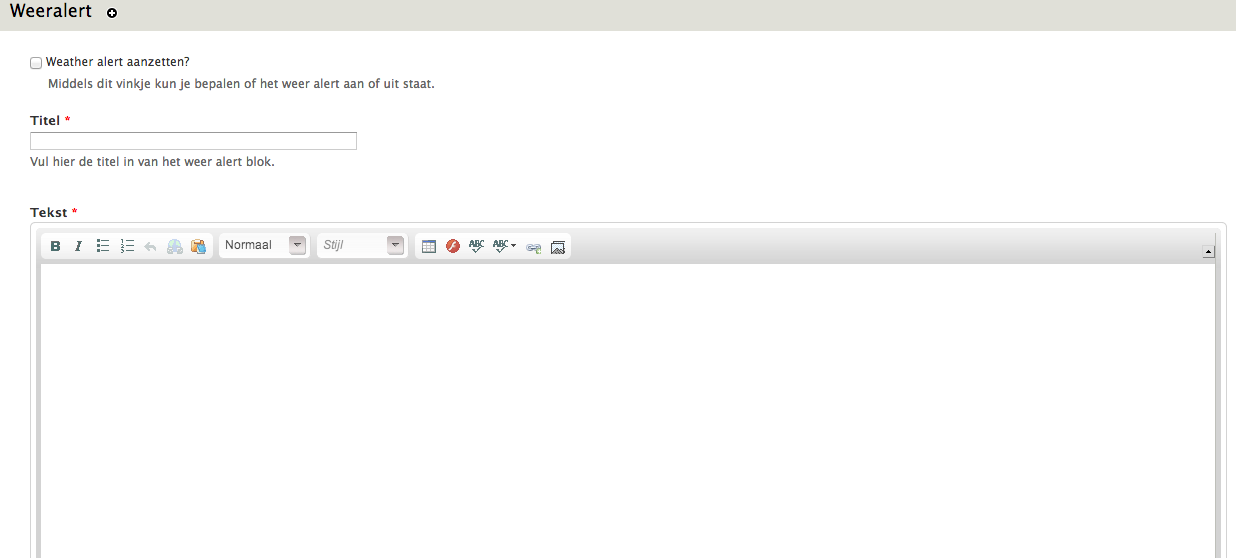
\includegraphics[width=\textwidth]{img/weeralert.png}
\end{center}

\subsubsection{Weer tekst}
De tekst bij de weersverwachting is te vinden bij het bewerken van die pagina in het "Intro" veld. Let erop dat de tekst niet in het bodyveld komt, want deze wordt overschreven door de import.

Tekst bij de kaart kan aangepast worden via de vertaalinterface: \drupalpath{/admin/config/regional/translate/translate}.